\documentclass[letterpaper,12pt]{scrartcl}
\usepackage[utf8]{inputenc}
\usepackage{amsmath}
\usepackage{amssymb}
\usepackage{graphicx}

\title{Amateur Radio Basic Qualification -- The Essentials}
\subtitle{Section Three: Equipment and Fundamentals}
\author{University of Waterloo Amateur Radio Club}
\date{\today}

\begin{document}

\maketitle
\tableofcontents

\section{Introduction}

These notes were prepared from Issue 3 of RIC-7 ``Basic Qualification Question Bank for Amateur Radio Operator Certificate Examinations'', published April 2007.
They cover 100\% of testable material on the Basic Qualification examination, but do not go beyond what is absolutely necessary to know in order to pass the examination.
The candidate is encouraged to perform their own research on topics that are not fully covered here.

\section{The Essentials: Section Three}

\subsection{Components of an HF Station}

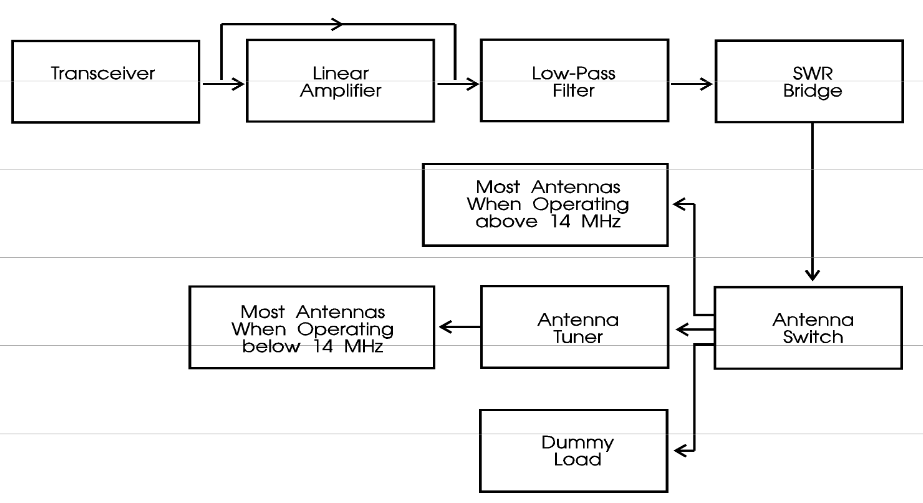
\includegraphics[width=150mm]{hf-station.png}

\subsection{Frequency Modulation Transmitter}

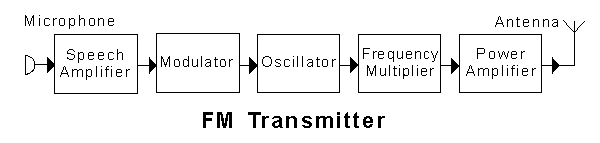
\includegraphics[width=150mm]{fm-transmitter.png}

\subsection{Frequency Modulation Receiver}

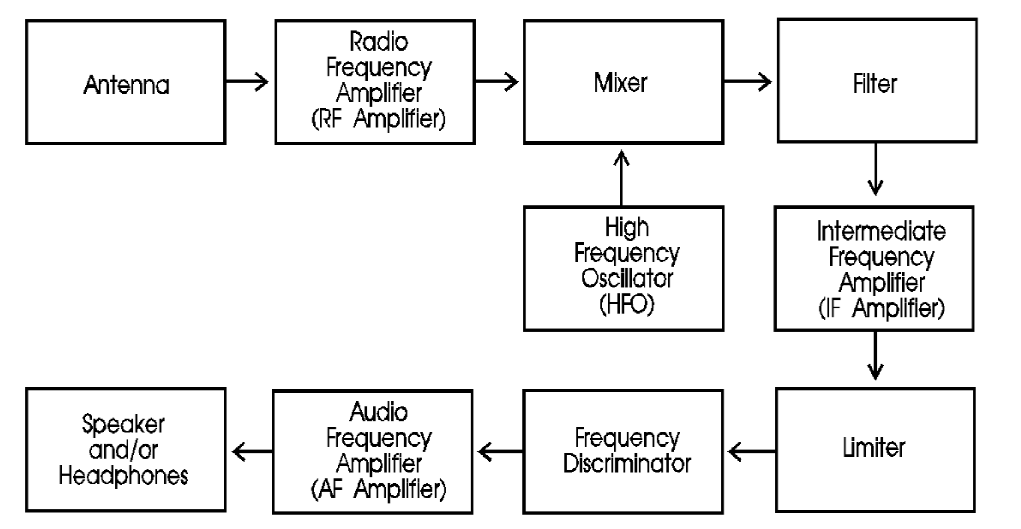
\includegraphics[width=150mm]{fm-receiver.png}

\subsection{CW Transmitter}

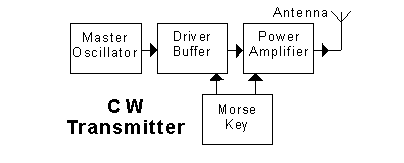
\includegraphics[width=150mm]{cw-transmitter.png}

\subsection{CW/SSB Receiver}

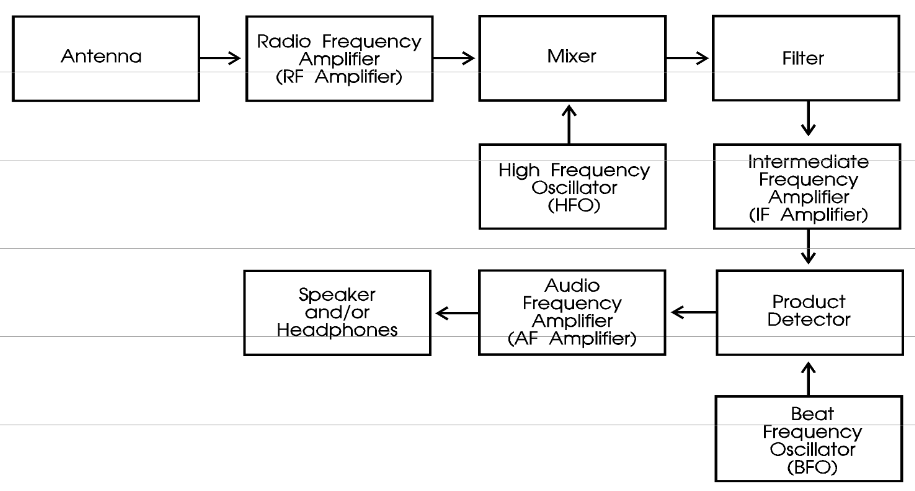
\includegraphics[width=150mm]{cw-ssb-receiver.png}

\subsection{SSB Transmitter}

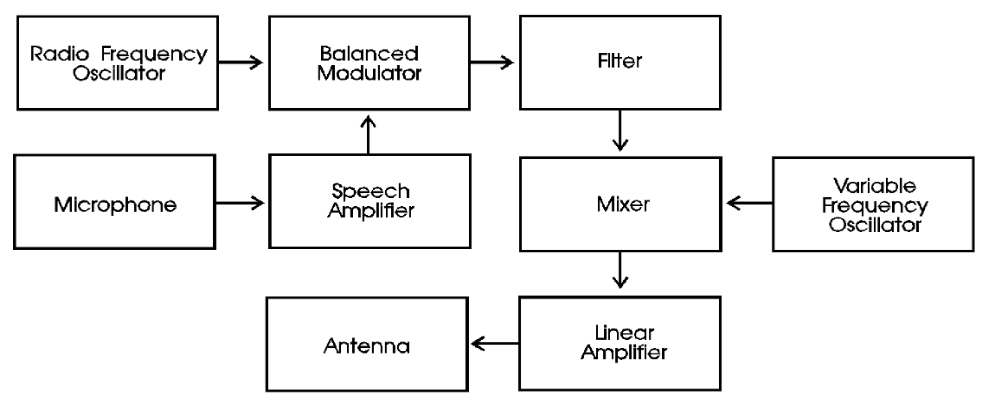
\includegraphics[width=150mm]{ssb-transmitter.png}

\subsection{Digital System}

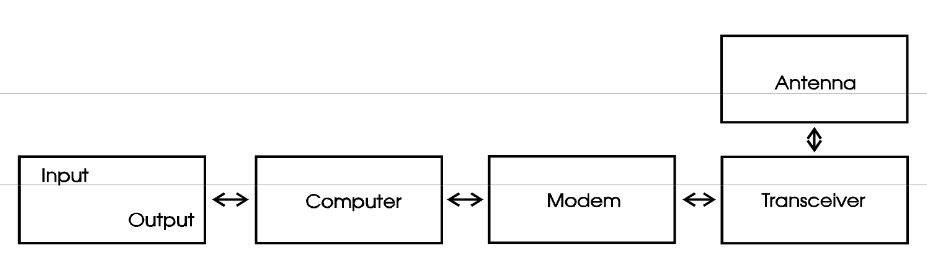
\includegraphics[width=150mm]{digital-system.png}

\subsection{Power Supply}

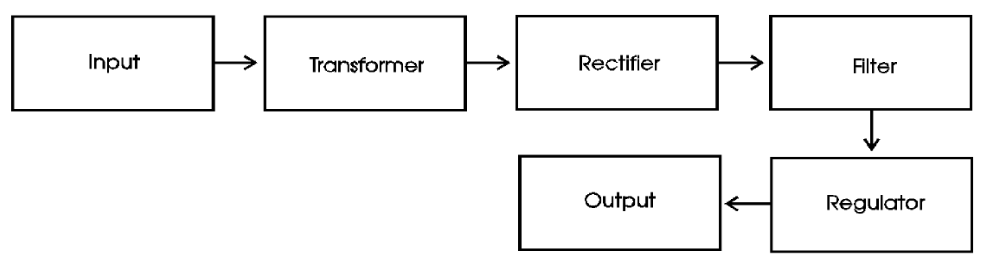
\includegraphics[width=150mm]{power-supply.png}

\subsection{Yagi-Uda Antenna}

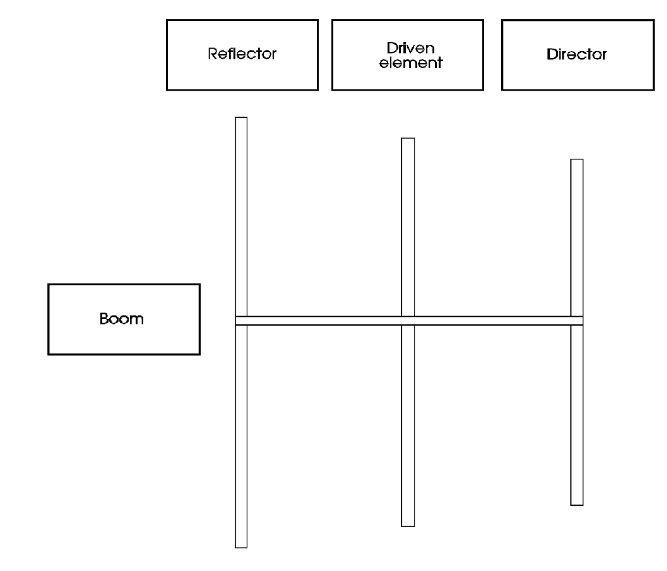
\includegraphics[width=150mm]{yagi-uda.png}

\subsection{Receiver Fundamentals}

\begin{itemize}
\item The three main parameters against which the quality of a receiver is measured are \textbf{sensitivity}, \textbf{selectivity}, and \textbf{stability}.
\item In order from narrowest to widest bandwidth, typical radio emissions you might receive are CW, RTTY, SSB voice, and FM voice.
\item The bandwidth of CW is about 250~Hz. A typical carrier frequency for CW is between 750 and 850~Hz.
\item The bandwidth of single sideband is about 2.4~kHz.
\item Signal-plus-noise to noise ratio (or just signal-to-noise ratio) is a measure of a receiver's sensitivity.
\item If two receivers of different sensitivity are compared, the less sensitive receiver will produce less signal or more noise.
\item Single sideband suppressed carrier is usually detected with a product detector.
\item A receiver designed for SSB reception must have a beat frequency oscillator (BFO) because the suppressed carrier must be replaced for detection.
\item A notch filter is a very, very narrow band-stop filter; its function is to attenuate a specific frequency as much as possible.
A notch filter can be used to attenuate an interfering carrier signal when receiving an SSB transmission.
\end{itemize}

\subsection{Transmitter Fundamentals}

\begin{itemize}
\item \textbf{Chirp} is a small, audible change in a transmitter's frequency each time it is keyed. A malfunctioning CW transmitter may exhibit chirp that can be heard on air
as a shift in the carrier tone. To keep such a transmitter from chirping, the power supply voltages must be kept very steady.
\item A VFO-controlled transmitter has a variable-frequency oscillator connected to a driver and a power amplifier.
\item Amplitude modulation is a scheme that changes the amplitude of an RF wave for the purpose of conveying information.
\item Morse code is usually transmitted by radio as an interrupted carrier.
\item A mismatched antenna or feedline may present an incorrect load to the transmitter. 
Since less than 100\% of the power from the power amplifier will be transmitted to the load, the antenna will not radiate with as much energy
as with a proper matching. Additionally, the ``lost'' power will be reflected back through the feedline and dissipated as heat.
The result may be excessive heat produced in the final transmitter stage or in the cable.
\item An RF oscillator should be electrically and mechanically stable. This is to ensure that the oscillator does not drift in frequency.
\end{itemize}

\subsection{Single Sideband}

\begin{itemize} 
\item An SSB transmitter that is operated with the microphone gain set too high will cause splatter interference to other stations operating near its frequency.
The same result will be observed if too much speech processing is used.
\item \textbf{Peak envelope power} is the average power supplied to an antenna transmission line during one RF cycle at the crest of the modulation envelope.
\item Suppressing the carrier in a double-sideband phone transmission means that more power can be put into the sidebands
(because the carrier contains no useful information).
\item The automatic level control (ALC) in an SSB transmitter controls the peak
audio input so that the final amplifier is not overdriven.
The microphone gain control should be adjusted on a single-sideband phone transmitter for slight movement of the ALC meter on modulation peaks.
\end{itemize}

\subsection{Frequency Modulation}

\begin{itemize}
\item If an FM transmitter is operated with the microphone gain or deviation set too high, it may cause interference to other stations
operating near its frequency. This is called ``overdeviation''. If this is happening to you, talk farther away from the microphone or turn down the mic gain.
\item An FM transmitter with a broken microphone produces an unmodulated carrier.
\item FM voice is best for local VHF/UHF radio communications because it has high-fidelity audio which can be understood even when the signal is somewhat weak.
\item The usual bandwidth of a frequency-modulated amateur signal is between 10 and 20~kHz.
FM phone cannot be used below 29.5~MHz because the bandwidth would exceed limits in the regulations.
\item FM receivers perform in an unusual manner when two or more stations are present. The loudest signal, even though it is only two or three times 
as loud as the other signals, will be the only transmission demodulated. This is called the \textbf{capture effect}.
\end{itemize}

\subsection{Voice and CW Operation}

\begin{itemize}
\item Many amateurs use an electronic keyer to help form good Morse code characters.
\item It is a good idea to tune with a dummy load to reduce interference on the air. You can expect a dummy load to get warm when in use because
it is essentially a giant resistor and dissipates RF energy as heat.
\item A ``VOX'' circuit causes a transmitter to automatically transmit when an operator speaks into its microphone.
\item A properly adjusted speech processor on a single-sideband transmitter will improve speech intelligibility at the receiver.
If a single-sideband phone transmitter is 100\% modulated, a speech processor will add nothing to the output power.
\item When switching from receive to transmit, the receiver should be muted \textit{first}, before the transmitter is enabled.
This is a safety interlock that will save you from blowing up your receiver's front end.
\item A speaker and a microphone are electrically identical. Yelling into a loudspeaker will cause it to function as a microphone, and vice versa.
\end{itemize}

\subsection{Digital Operation}

\begin{itemize}
\item A packet radio link is ``connected'' when a transmitting station is sending data to only one receiving station, which replies
that the data is being received correctly.
\item A packet radio station is ``monitoring'' when it is displaying messages that may not be sent to it and is not replying to any message.
\item A \textbf{digipeater} is a packet radio station that retransmits only data that is marked to be retransmitted.
\item A packet radio network connects multiple stations so that data can be sent over long distances.
\item In packet radio, a transceiver and computer system are connected to a ``terminal node controller'' (TNC).
The easiest and simplest way to accomplish this is to connect the TNC to the transceiver's microphone input and speaker/headphone output.
Packet radio uses the ASCII encoding to express letters and numbers as digital information, and may also use a protocol called AX.25
to provide network control and link-level operations.
\item RTTY communications should maintain a frequency separation of 250 to 500~Hz (center to center) from contacts in progress to minimize interference.
\item Digital transmissions use signals called ``mark'' and ``space'' to transmit the states 1 and 0.
\item AMTOR transmissions can be made in two modes. Mode A uses the ``Automatic Repeat Request (ARQ)'' protocol, and is normally used for
communications after contact has been established (Mode B is faster but less reliable and is used for making calls).
\item VHF packet communications most commonly use a data rate of 1200 baud. There is a very good reason for this. 
Most packet communications on VHF are done through a mode called ``Audio Frequency Shift Keying (AFSK)'', which
uses audible frequencies transmitted and received directly through the microphone and speaker. There is an upper limit on the frequency of audio that can be passed
through a VHF transceiver (in order to maintain maximum bandwidth of the modulated signal), and using a higher data rate would necessitate
the use of audio frequencies that would cause overdeviation of the transmitter.
\end{itemize}

\subsection{Introduction to Electricity}

\begin{itemize}
\item Current is the flow of electrical charge in a circuit. The symbol for current is $I$.
\item Current is measured ``through'' a point in the circuit.
\item The unit of current is the ampere or amp.
\item There are two types of current. \textbf{Direct current (DC)} flows in one direction and does not vary with time; \textbf{alternating current (AC)} changes direction and varies
with time (usually sinusoidally).
\item A battery is a source of ``EMF'', or electromotive force. This is also known as ``voltage''.
\item A lot of hams use the symbol $E$ for voltage. From an engineering point of view, this is completely wrong.
Despite all evidence to the contrary that you may find in ham radio literature, the symbol for voltage is and has always been $V$.
\item Voltage is measured as a ``potential difference'', across two points in a circuit.
\item The unit of voltage is the volt.
\item A standard automobile battery supplies about 12 volts. An important distinction between this type of battery (a ``lead acid battery'') and a conventional flashlight
battery is that the lead acid battery can be repeatedly recharged.
\item All batteries have an internal resistance, which essentially behaves as a resistor in series with the battery.
This internal resistance can cause the supplied voltage of the battery to drop when the current is high.
\item Batteries should never be short-circuited (connecting the terminals directly to each other).
\item All batteries have discharge limits. Nickel-cadmium batteries should not be discharged to less than 1.0 volts per cell.
% FIXME \bogus Diagrams of series and parallel circuits
\item To increase the current capacity of a cell, several cells should be connected in parallel. To increase the voltage output, several cells should be connected in series.
\end{itemize}

\subsection{Power Supplies Again}

\begin{itemize}
\item Power is the amount of energy per unit time delivered to a device. 
The symbol for power is $P$.
\item Power is measured in watts.
\item The power delivered to an electrical device such as a resistor 
is equal to the voltage across its terminals multiplied by the current passing through it: $P = IV$.
Knowing how to calculate power is important for determining what components to use -- for example,
most resistors have a specified ``maximum power'', and if more power is put through the resistor than the maximum,
the resistor will blow up. The same is true of power supplies. If you want to supply 12 volts of power at 5 amperes of current,
your power supply must be rated higher than 60 watts for safe operation.
\item If your mobile transceiver works in your car but not in your home, the first thing to check is the power supply.
\item A power supply converts household current (AC) into 12-volt DC.
\item Transceivers usually need lots of power and therefore require heavy-duty power supplies.
\item The diode is an important part of a simple power supply, and you will learn more about it in the section on semiconductors.
It converts AC to DC, since it allows electrons to flow in only one direction (from cathode to anode).
\item Power line voltages have been made standard over the years, and the voltages generally supplied to homes
are approximately 120 and 240 volts. Power lines in North America provide alternating current power at a frequency of 60~Hz.
\item So-called ``transformerless'' power supplies are used in some applications. When working on such equipment, one should be
very careful because one side of the line cord is connected to the chassis.
\item An autotransformer can be used as an efficient method of increasing or decreasing a voltage. They are especially useful in areas
with poor electrical service when wall voltages are consistently high or low.
\item Since power supplies use low-frequency alternating current, a very loud low-frequency hum in a transmission is almost certainly
coming from the power supply.
\end{itemize}

\subsection{Electricity Safety}

\begin{itemize}
\item The best way to keep unauthorized individuals from using an amateur station at home is to use a key-operated on/off switch in the main power line.
\item To lock out a mobile station, disconnect the microphone and lock it up when not in use.
\item High-voltage power supplies often use a safety interlock consisting of a switch that breaks contact if the case is opened. This is to prevent
anyone opening the cabinet from coming into contact with dangerous high voltages.
\item As little as 0.1~A of current can be fatal to the human body.
\item The heart is especially sensitive to very small amounts of electrical current, and can be fatally affected.
\item The minimum voltage which is usually dangerous to humans is 30~V.
\item If you discover someone being burned by high voltage, don't touch them or the wires; turn off the power, call for emergency help,
and give CPR if needed.
\item The safest method to remove an unconscious person from contact with a high voltage source is \textit{turning off the power first}.
\item The safest way to work on a transmitter or a power supply is \textit{turning off the power first}.
\end{itemize}

\subsection{Electrical Ground}

\begin{itemize}
\item For best protection from electrical shock, all station equipment should be ``grounded''. This means that the chassis of the equipment is connected with a wire to an electrical ground.
This can be a cold water pipe or an ``earthing rod'' driven into the ground.
\item Earthing rods are typically made of copper-clad steel for superior electrical conductivity.
\item A long ground wire can act like an antenna; this is especially notorious on HF bands, where stations that are in tall buildings are installed
with long ground wires that are resonant on several HF bands and radiate RF energy, resulting in inexplicable RF burns.
It is recommended to keep ground wires as short as possible.
\item On mains-operated power supplies, the ground wire should be connected to the metal chassis of the power supply.
This ensures that in case there is a fault in the power supply, the chassis does not develop a high voltage with respect to the ground.
\item The purpose of using a three-wire power cord and plug on amateur radio equipment is to prevent the chassis from becoming live
in case of an internal short (the third prong on the plug is a ground connection).
\end{itemize}

\subsection{Antenna, Tower, and Lightning Safety}

\begin{itemize}
\item All antenna and rotor cables should be grounded when not in use to protect the station and building from lightning damage.
\item When working on an antenna tower, it is necessary to wear approved equipment in accordance with provincial safety standards concerning climbing.
\item A safety belt should be worn when working on an antenna tower to prevent you from accidentally falling.
\item A hard hat should be worn when working on an antenna tower to protect your head from something dropped from the tower.
\item Horizontal wire antennas should be placed high enough so that no one can touch any part of the antenna from the ground.
Touching an antenna can cause RF burns.
\item Before beginning repairs on an antenna, turn off the transmitter and disconnect the feedline.
\end{itemize}

\subsection{Radiation Safety}

\begin{itemize}
\item When operating at 1200~MHz or above, keep the antenna away from your eyes when RF is applied. These frequencies are microwave and can cause tissue damage to your eyes.
\item Before removing the shielding on a power amplifier, make sure the amplifier cannot accidentally be turned on.
\item You should make sure the antenna of a handheld transceiver is not close to your head when transmitting in order to reduce your exposure to RF energy.
The antenna should be positioned away from your head and away from others.
\item Exposure to a large amount of RF energy will heat body tissue. The eyes are the most likely to be damaged from the heating effects of RF radiation.
\item If you operate your amateur station with indoor antennas, locate them as far away as possible from living spaces that will be occupied while you are operating.
\item Directional high-gain antennas should be mounted higher than nearby structures so they will not direct
RF energy toward people in those structures.
\item The ends and center of a dipole antenna should be as high as possible to prevent people from coming into contact with the antenna.
\end{itemize}

\end{document}

